\documentclass{beamer}
%Information to be included in the title page:

\usepackage{amsmath, mathtools, tikz}
\usetikzlibrary{calc, positioning}

\uselanguage{italian}
\languagepath{italian}
\deftranslation[to=italian]{Definition}{Definizione}
\deftranslation[to=italian]{Theorem}{Teorema}
\deftranslation[to=italian]{Proposition}{Proposizione}

\deftranslation[to=italian]{Example}{Esempio}

\newenvironment{exercise}[1][]
{
  \begin{exampleblock}{Esercizio (#1)}
}
{
  \end{exampleblock}
}



\AtBeginSection[]{
  \begin{frame}
    \frametitle{Outline}
    \tableofcontents[currentsection]
  \end{frame}
}



\newcommand{\Hom}{\mathrm{Hom}}
\newcommand{\im}{\mathrm{im}\,}
\newcommand{\obj}{\mathrm{obj}}
\newcommand{\Vertk}{\mathrm{Vert}}
\newcommand{\Dr}[1]{\ensuremath{\underset{#1}{\textnormal{Dr}}}}

\newcommand{\ssedef}{\mathrel{\stackrel{\mathrm{def}}{\Leftrightarrow}}}

\newcommand{\cat}[1]{\mathrm{\mathbf{#1}}}

\usetheme{Warsaw}
\usefonttheme[onlymath]{serif}

\addtobeamertemplate{navigation symbols}{}{%
    \usebeamerfont{footline}%
    \usebeamercolor[fg]{footline}%
    \hspace{1em}%
    \insertframenumber/\inserttotalframenumber
}

\title{Coomologia di Čech}
\author{Dario Di Meo, D70000023}
\date{Esame di Geometria Algebrica, XX/12/25}

\begin{document}

\frame{\titlepage}

\section{Coomologia di fasci}
\subsection{Successioni di oggetti e morfismi}

\begin{frame}{Insiemi parzialmente ordinati come categorie}
    Sia $(X,\preceq)$ un insieme parzialmente ordinato.
    \pause

    È possibile considerarlo come una categoria $\mathcal{X}$ ponendo:
    \pause
    \begin{itemize}
        \item $\obj(\mathcal{X})=X$;
    \pause
        \item $\Hom(x,y)=
        \begin{cases}
            \emptyset & \text{se $x\npreceq y$} \\
            \{\iota^x_y\} & \text{se $x\preceq y$}
        \end{cases}$ per ogni $x,y\in\obj(\mathcal{X})$;
    \pause
        \item $\iota_y^x\cdot\iota_z^y=\iota_z^x$ se $x\preceq y\wedge y\preceq z$.
    \end{itemize}
\end{frame}

\begin{frame}{Insiemi parzialmente ordinati come categorie}
    
    \begin{example}[Topologia di uno spazio topologico]
        Sia $(X,\tau)$ uno spazio topologico. $(\tau,\subseteq)$ è parzialmente ordinato quindi può vedersi come una categoria i cui oggetti sono gli aperti e i cui morfismi sono le inclusioni.
    \end{example}
    \pause
        \begin{example}[Interi con diseguaglianze contrarie]
        Poniamo $n\preceq m\ssedef m\leq n$.
        \pause
        $(\mathbb{Z},\preceq)$ è totalmente ordinato, quindi parzialmente ordinato, e può vedersi come la categoria i cui oggetti sono gli interni e i cui morfismi sono le disuguaglianze contrarie:
        $$\cdots\longrightarrow\underset{n+1}{\bullet}\longrightarrow\underset{n}{\bullet}\longrightarrow\underset{n-1}{\bullet}\longrightarrow\cdots$$
    \end{example}
\end{frame}

\begin{frame}{Successioni di oggetti e morfismi}
    \begin{definition}[Successioni di oggetti e morfismi]
        Sia $\mathcal{C}$ una categoria.
        \pause

        Una \textbf{successione di oggetti e morfismi}, o \textbf{successione}, è un funtore covariante $S:\mathbb{Z}\rightarrow\mathcal{C}$:
        $$\cdots\longrightarrow A_{n+1}\xrightarrow{f_{n+1}}A_n\xrightarrow{f_n}A_{n-1}\longrightarrow\cdots$$
    \end{definition}

    \begin{block}{Osservazione}
        Analogamente, definiamo una \textbf{successione finita di oggetti e morfismi} di $\mathcal{C}$ come un funtore covariante
        $F:\mathrm{\mathbf{n+1}}\rightarrow\mathcal{C}$.
    \end{block}
\end{frame}

\begin{frame}{Successioni esatte}
    \begin{definition}[Successione esatta]
        Sia $A$ un anello commutativo.
        \pause

        Una successione finita o infinita di $A$-omomorfismi e $A$-moduli
        $$\cdots\longrightarrow M_{n+1}\xrightarrow{f_{n+1}}M_n\xrightarrow{f_n}M_{n-1}\longrightarrow\cdots$$
        si dice \textbf{successione esatta} se $\im f_{n+1}=\ker f_n$ per ogni $n$.
    \end{definition}
    \pause
    \begin{definition}[Successione esatta corta]
        Una \textbf{successione esatta corta} è una successione esatta della forma
        $$0\rightarrow A\xrightarrow{f}B\xrightarrow{g}C\rightarrow0$$
    \end{definition}
\end{frame}

\subsection{Categorie abeliane}
\begin{frame}{Categorie additive}
\begin{definition}[Categoria additiva]
    Una categoria $\mathcal{C}$ si dice \textbf{additiva} se
    \pause
    \begin{enumerate}[i.]
        \item $\Hom(A,B)$ è un gruppo abeliano per ogni $A,B\in\obj(C)$;
        \pause
        \item Vale la proprietà distribuitva sui morfismi: \pause dati
        $$X\xrightarrow{a}A\underset{g}{\overset{f}{\rightrightarrows}}B\xrightarrow{b}Y$$
        allora $(f+g)\cdot b=f\cdot b+g\cdot b$ e $a\cdot(f+g)=a\cdot f+a\cdot g$;
        \pause
        \item $\mathcal{C}$ ha un oggetto zero;
        \pause
        \item $\mathcal{C}$ ha prodotti finiti e coprodotti finiti.
    \end{enumerate}
\end{definition}
\end{frame}

\begin{frame}{Categorie additive}
    \begin{definition}[Funtore additivo]
        Siano $\mathcal{C}$ e $\mathcal{D}$ categorie additive.
        \pause

        Un funtore $F:\mathcal{C}\rightarrow\mathcal{D}$ si dice \textbf{additivo} se per ogni $A,B\in\obj(\mathcal{C})$ e per ogni $f,g\in\Hom(A,B)$ si ha
        $$F(f+g)=F(f)+G(g)$$
    \end{definition}
\end{frame}

\begin{frame}{Categorie abeliane}
    \begin{definition}[Categoria abeliana]
     Sia $\mathcal{C}$ una categoria. È abeliana se
    \pause
    \begin{enumerate}[i.]
        \item Ogni morfismo ha un kernel e un cokernel;
        \pause
        \item Ogni monomorfismo è un kernel e ogni epimorfismo è un cokernel.
    \end{enumerate}   
    \end{definition}
    \pause
    \begin{lemma}
        $\cat{Ab}$ è una categoria abeliana.
    \end{lemma}

\end{frame}


\begin{frame}{Risoluzioni iniettive}
\begin{definition}[Oggetti proiettivi]
Siano $\mathcal{A}$ una categoria abeliana e $E\in\obj(\mathcal{A})$.
\pause

$E$ si dice \textbf{iniettivo} se per ogni monomorfismo $g:A\rightarrow B$ e per ogni morfismo $f:A\rightarrow E$, esiste $h:B\rightarrow E$ tale che $f=g\cdot h$.
\pause
Equivalentemente, $h$ rende commutativo il seguente diagramma:
\[
        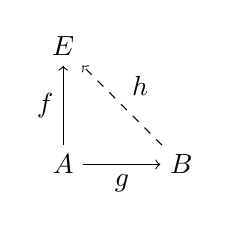
\begin{tikzpicture}[->, node distance=1.5cm]
        \node (E) {$E$};
        \node (A) [below of=E] {$A$};
        \node (B) [right of=A] {$B$};

        \draw (A) -- (E) node[midway, left] {$f$};
        \draw (A) -- (B) node[midway, below] {$g$};
        \draw[dashed] (B) -- (E) node[midway, above right] {$h$};

        \end{tikzpicture}
        \]
\end{definition}    
\end{frame}

\begin{frame}{Risoluzioni iniettive}
    \begin{definition}[Risoluzione iniettiva]
        Siano $\mathcal{A}$ una categoria abeliana e $A\in\obj(\mathcal{A})$.
        \pause
        Una \textbf{risoluzone iniettiva di $A$} è una successione esatta
        $$\mathrm{\mathbf{E}}=0\longrightarrow A\xrightarrow{\eta}E^0\xrightarrow{d^0}E^1\xrightarrow{d^1}E^2\longrightarrow\cdots$$
        con $E^n$ iniettivo per ogni $n\in\mathbb{N}_0$.
    \end{definition}
    \pause
    \begin{definition}[Risoluzione ineittiva troncata]
        Alla risoluzione iniettiva $\mathrm{\mathbf{E}}$ è possibile associare il complesso
        $$\mathrm{\mathbf{E}}^A=0\longrightarrow E^0\xrightarrow{d^0}E^1\xrightarrow{d^1}E^2\longrightarrow\cdots$$
        detto \textbf{risoluzione iniettiva troncata}.
    \end{definition}
\end{frame}

\subsection{Fasci}
%Riassumiamo l'argomento di Nino:
\begin{frame}{Fasci di gruppi abeliani}
    \begin{definition}[Fascio di gruppi abeliani]
    Sia $(X,\tau)$ uno spazio topologico. 
    \pause
    Un \textbf{fascio di gruppi abeliani su $X$} è un funtore controvariante
    $$\mathcal{F}:\tau\rightarrow\mathrm{\mathbf{Ab}}$$
    tale che:
    \pause
    \begin{itemize}
        \item Ad ogni aperto $A$ associa un gruppo abeliano $\mathcal{F}(A)$;
        \pause
        \item A $\iota_B^A$ associa $\mathcal{F}(\iota_B^A)=\rho_B^A\in \Hom(\mathcal{F}(B),\mathcal{F}(A))$;
        \pause
        \item Per ogni famiglia di aperti $\{A_i\}_{i\in I}$ e per ogni famiglia $\{a\}_{i\in I}$ tale che $a_i\in \mathcal{F}(A_i)$ per ogni $i$, se ${a_i}_{|A_i\cap A_j}={a_j}_{|A_i\cap A_j}$, allora esiste ed è unico $a\in \mathcal{F}\left(\bigcup_{i}A_i\right)$ tale che $a_{|A_i}=a$ per ogni $i$.
    \end{itemize}
    \end{definition}
\end{frame}

\begin{frame}{La categoria dei fasci di gruppi abeliani}
    I fasci di gruppi abeliani costituiscono una categoria. In particolare, dato uno spazio topologico $(X,\tau)$:
    \pause
    \begin{definition}[Categoria dei fasci di gruppi abeliani]
        Definaimo $\mathrm{\mathbf{Sh}}(X,\mathrm{\mathbf{Ab}})$ come la categoria tale che:
        \pause
        \begin{itemize}
            \item $\obj(\cat{Sh}(X,\cat{Ab}))$ è costituito dai fasci $\tau\rightarrow\cat{Ab}$;
            \pause
            \item $\Hom(\mathcal{F},\mathcal{G})$ è costutito dalle trasformazioni naturali $\mathcal{F}\rightarrow\mathcal{G}$.
        \end{itemize}
    \end{definition}
    \pause
    \begin{lemma}
        $\cat{Sh}(X,\cat{Ab})$ è una categoria abeliana.
    \end{lemma}
\end{frame}

\begin{frame}{Fasci di gruppi abeliani}
    \begin{definition}[Funtore delle sezioni globali]
        Il \textbf{funtore delle sezioni globali} è il funtore covariante additivo
        $$\Gamma:\mathrm{\mathbf{Sh}}(X, \mathrm{\mathbf{Ab}})\rightarrow\mathrm{\mathbf{Ab}}$$
        tale che
        \pause
        \begin{itemize}
            \item Ad ogni fascio $\mathcal{F}$ su $X$, associa $\mathcal{F}(X)$;
        \pause
            \item Al morfismo di fasci $\varphi:\mathcal{F}\rightarrow\mathcal{G}$ associa $\varphi_X:\mathcal{F}(X)\rightarrow\mathcal{G}(X)$.
        \end{itemize}
    \end{definition}
\end{frame}


\begin{frame}{Coomologia di fasci}
    \begin{definition}[Coomologia di fasci]
        Siano $X$ uno spazio topologico e $\mathcal{F}$ un fascio di gruppi abeliani.
        \pause

        Consideriamo una risoluzione iniettiva di $\mathcal{F}$ 
        $$\mathrm{\mathbf{E}}=0\longrightarrow\mathcal{F}\xrightarrow{\eta}\mathcal{E}^0\xrightarrow{d^0}\mathcal{E}^1\xrightarrow{d^1}\mathcal{E}^2\longrightarrow\cdots$$
        Allora:
        \pause
        $$H^q(\mathcal{F})\coloneq H^q\left(\Gamma{\mathrm{\mathbf{E}}}^\mathcal{F}\right)=\frac{\ker\left(\Gamma(d^q):\Gamma(\mathcal{E}^q)\rightarrow\Gamma({\mathcal{E}}^{q+1})\right)}{\im\left(\Gamma(d^{q-1}):\Gamma(\mathcal{E}^{q-1})\rightarrow\Gamma({\mathcal{E}}^{q})\right)}$$

    \end{definition}
\end{frame}

\section{Coomologia di Čech}



\begin{frame}
    \begin{block}{Definizione (Complesso simpliciale astratto)}
    Un complesso simpliciale astratto $K$ è una coppia
    $$K=\left(\Vertk(K),\mathcal{S}\right)$$
    dove
    \begin{enumerate}
        \item $\Vertk(K)$ è un inieme non vuoto di elementi chiamati vertici;
        \item $\mathcal{S}$ è un sottoinsieme di parti finite e non vuote $\sigma$ di $\Vertk(K)$ chiamate simplessi tali che
        \begin{enumerate}[(a)]
            \item Per ogni $v\in\Vertk(K)$, $\{v\}\in\mathcal{S}$;
            \item $\sigma\in\mathcal{S}\wedge\tau\subseteq\sigma\wedge\tau\ne\emptyset\Rightarrow\tau\in\mathcal{S}$.
        \end{enumerate}
    \end{enumerate}
    Se $\sigma$ è un simplesso e $|\sigma|=n+1$, $\sigma$ è detto $n$-simplesso.

    \end{block}
\end{frame}





\begin{frame}
    \begin{block}{Definzione (Nervo)}
        Sia $X$ uno spazio topologico e sia $\mathcal{U}$ un suo rivestimento aperto. Si dice nervo $N(\mathcal{U})$ il complesso simpliciale astratto i cui vertici sono gli aperti del ricoprimento e i simplessi le sottofamiglie finite di $\mathcal{U}$ la cui intersezione è non vuota, cioè
    $\Vertk(N(\mathcal{U}))=\mathcal{U}$
    e
    $$\mathcal{S}=\Bigg\{(U_{i_0},U_{i_1},...,U_{i_n}):n\in\mathbb{N}_0\wedge\bigcap_{j=0}^nU_{i_j}\ne\emptyset\Bigg\}$$

    Indichiamo con $\Sigma_q$ l'insieme dei $q$-simplessi nel nervo.

    \end{block}
\end{frame}

\begin{frame}
    \begin{block}{Definizione (Complesso di gruppi di cocatene)}
        Definiamo il seguente complesso di gruppi e omomorfismi
        $$C^\bullet(N(\mathcal{U}),\mathcal{F})=\cdots\longrightarrow C^q(\mathcal{U},\mathcal{F})\xrightarrow{\delta^q}C^{q+1}(\mathcal{U},\mathcal{F})\longrightarrow\cdots$$
        dove:
        \pause
        $C^q(\mathcal{U},\mathcal{F})= \Dr{\sigma\in\Sigma_q}\mathcal{F}\left(\bigcap \sigma\right)$
        \pause
        e, presa $f:\Sigma_q\rightarrow\bigcup_{\sigma\in\Sigma_q}\mathcal{F}\left(\bigcap\sigma\right)$ in $C^q(\mathcal{U},\mathcal{F})$:
        
        $$\delta^q(f)=\left(\sigma\in\Sigma_{q+1}\mapsto\sum_{i=0}^{q+1}(-1)^i f\left(\hat{\sigma}^i\right)\in\bigcup_{\sigma\in\Sigma_{q+1}}\mathcal{F}\left(\bigcap\sigma\right)\right)$$
    
        in $C^{q+1}(\mathcal{F},\mathcal{U})$.
    \end{block}
\end{frame}

\begin{frame}

\begin{block}{Definizione (Gruppi di coomologia di un ricoprimento aperto con coefficienti in un fascio)}
    Siano $X$ uno spazio topologico, $\mathcal{U}$ un suo ricoprimento aperto e $\mathcal{F}$ un fascio di gruppi abeliani.
    \pause

    Chiamiamo \textbf{gruppi di coomologia} di $\mathcal{U}$ con coefficienti in $\mathcal{F}$, e li indichiamo con
    $$\check{H}^q(\mathcal{U},\mathcal{F})$$
    i gruppi di omologia del complesso $C^\bullet(N(\mathcal{U}),\mathcal{F})$.
\end{block}

\end{frame}

\subsection{Limiti diretti}

\begin{frame}
    \begin{definition}[Sistema diretto]
        Siano $(I,\preceq)$ un insieme parzialmente ordinato e $\mathcal{C}$ una categoria. 
        \pause
        
        Un \textbf{sistema diretto} in $\mathcal{C}$ su $I$ è una coppia ordinata
        $$\{M_i,\varphi^i_j\}\coloneq\left((M_i)_{i\in I},(\varphi^i_j)_{i\preceq j}\right)$$
        dove \pause $(M_i)_{i\in I}\subseteq\obj(\mathcal{C})$; \pause $(\varphi^i_j)_{i\preceq j}\subseteq {M_j}^{M_i}$ con $\varphi^i_i=\iota_{M_i}$ per ogni $i$; \pause per ogni $i\preceq j\preceq k$, il seguente diagramma è commutativo:
        \[
        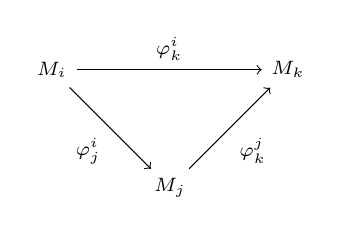
\begin{tikzpicture}[->, node distance=1.5cm, font=\scriptsize]
        \node (Mi) {$M_i$};
        \node (A) [right of=Mi] {};
        \node (Mk) [right of=A] {$M_k$};
        \node (Mj) [below of=A] {$M_j$};

        \draw (Mi) -- (Mk) node[midway, above] {$\varphi^i_k$};
        \draw (Mi) -- (Mj) node[midway, below left] {$\varphi^i_j$};
        \draw (Mj) -- (Mk) node[midway, below right] {$\varphi^j_k$};

        \end{tikzpicture}
        \]
    \end{definition}
\end{frame}

\begin{frame}
    \begin{definition}[Limite diretto] % insertion morfisms
        Siano $(I,\preceq)$ un poset, $\mathcal{C}$ una categoria e $\{M_i,\varphi^i_j\}$ diretto in $\mathcal{C}$. 
        \pause
        
        Il \textbf{limite diretto} è una coppia costituita da un oggetto $\varinjlim M_i$ e da una famiglia di morfismi $(\alpha_i)_{i\in I}\subseteq (\varinjlim M_i)^{M_i}$ tali che:
        \begin{enumerate}[i]
            \pause
            \item $\varphi^i_j\cdot\alpha_j=\alpha_i$ quando $i\preceq j$;
            \pause
            \item Presi $X\in\obj(\mathcal{C})$ e dei morfismi $f_i:M_i\rightarrow X$ tali che $\varphi^i_j\cdot f_j=f_i$ per ogni $i\preceq j$, esiste ed è unico $\theta:\varinjlim M_i\rightarrow X$ che rende il seguente diagramma commutativo:
            \vspace{-0.4cm}
            \[
            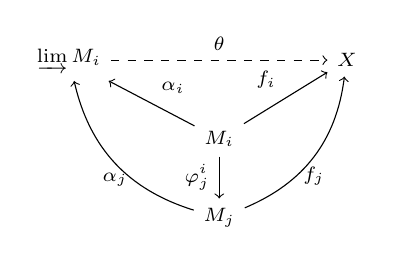
\begin{tikzpicture}[->, node distance=1cm, font=\scriptsize]
            \node (lim) {$\varinjlim M_i$};
            \node (A) [right=1.25cm of lim] {};
            \node (X) [right=1.25cm of A] {$X$};
            \node (Mi) [below of=A] {$M_i$};
            \node (Mj) [below of=Mi] {$M_j$};

            \draw[dashed] (lim) -- (X) node[midway, above] {$\theta$};
            \draw (Mi) -- (lim) node[midway, above right] {$\alpha_i$};
            \draw (Mi) -- (X) node[midway, above left] {$f_i$};
            \draw (Mi) -- (Mj) node[midway, left] {$\varphi^i_j$};
            \draw (Mj) to[bend left] node[midway, below] {$\alpha_j$} (lim);
            \draw (Mj) to[bend right] node[midway, below] {$f_j$} (X);

            \end{tikzpicture}
            \]
        \end{enumerate}        
    \end{definition}
\end{frame}

\begin{frame}{Classi dirette}
    \begin{definition}[Classe diretta]
        Una classe $\mathcal{K}$ si dice \textbf{classe diretta} se su di essa è definita una relazione $\preceq$ riflessiva, asimmetrica e transitiva e se per ogni $k,k'\in\mathcal{K}$ esiste $k*\in\mathcal{K}$ tale che $k\preceq k^*$ e $k'\preceq k^*$.
    \end{definition}
\pause
    \begin{definition}[Sottoclasse cofinale]
        Una sottoclasse $\mathcal{L}$ di $\mathcal{K}$ si dice \textbf{cofinale} in $\mathcal{K}$ se, per ogni $k\in\mathcal{K}$, esiste $l\in\mathcal{L}$ tale che $k\preceq l$.
    \end{definition}
\pause
    \begin{block}{Osservazione}
        È possibile definire i sistemi diretti a partire da una classe diretta in maniera analoga a come fatto a partire da un insieme di indici.
    \end{block}
\end{frame}

\begin{frame}{Limiti su classi dirette} % Una categoria è cocompleta se per ogni sistema diretto esiste il colimite
    \begin{definition}[Categoria cocompleta]
        Una categoria $\mathcal{C}$ si dice \textbf{cocompleta} se il limite diretto esiste per ogni sistema diretto in $\mathcal{C}$.
    \end{definition}
    \pause
    \begin{block}{Proposizione}
    Siano $\mathcal{K}$ una classe diretta, $\mathcal{C}$ una categoria cocompleta e $\{A_k,\varphi^k_j\}$ un sistema diretto in $\mathcal{C}$ su $\mathcal{K}$. Se due sottoclassi di $\mathcal{K}$, siano esse $\mathcal{L}$ e $\mathcal{M}$, sono insiemi e cofinali in $\mathcal{K}$, allora
    $$\varinjlim\nolimits_\mathcal{L}A_k\cong\varinjlim\nolimits_\mathcal{M}A_k$$
    \end{block}    
    \pause
    Cioè, sotto le ipotesi della proposizione, è possibile formare limiti diretti su classi dirette.
\end{frame}

\subsection{La classe diretta degli $\check{H}^q(\mathcal{U},\mathcal{F})$}

\begin{frame}{Raffinamenti}
    \begin{definition}[Raffinamento]
        Siano $X$ uno spazio topologico e $\mathcal{U}$,$\mathcal{V}$ due suoi ricoprimenti aperti.
        \pause

        $\mathcal{V}$ si dice \textbf{raffinamento} di $\mathcal{U}$, e si indica con $\mathcal{U}\preceq\mathcal{V}$, se, per ogni $V\in\mathcal{V}$, esiste $U\in\mathcal{U}$ tale che $V\subseteq U$.
    \end{definition}
    \pause
    \begin{definition}[Funzione di raffinamento]
        Siano $\mathcal{U}$ e $\mathcal{V}$ due ricoprimenti aperti di un certo spazio con $\mathcal{U}\preceq\mathcal{V}$.
        \pause

        Scegliere, al variare di $V\in\mathcal{V}$, $V\subseteq U_V\in\mathcal{U}$ definisce una funzione
        $$r:V\in\mathcal{V}\mapsto U_V\in\mathcal{U}$$
        detta \textbf{funzione di raffinamento}.
    \end{definition}
\end{frame}

\begin{frame}
    \begin{definition}[Ordine parziale sui gruppi di cocatene]
        Sia $\mathcal{F}$ un fascio di gruppi abeliani su uno spazio $X$.
        \pause
        
        Poniamo $\check{H}^q(\mathcal{U},\mathcal{F})\preceq\check{H}^q(\mathcal{V},\mathcal{F})$ se e solo se, per definizione, esiste una funzione di raffinamento $r:\mathcal{V}\rightarrow\mathcal{U}$.
        \pause

        (Si dimosta che) $\preceq$ è un ordine parziale sugli $\check{H}^q(\mathcal{U},\mathcal{F})$.
    \end{definition}
\end{frame}

\begin{frame}
    Sia $\mathcal{K}$ la classe (diretta) dei gruppi $\check{H}^q(\mathcal{U},\mathcal{F})$. \pause
    \begin{exercise}[Ricerca di un sottoinsieme cofinale in $\mathcal{K}$]
        Sia $\mathcal{U}$ un ricoprimento aperto di $(X,\tau)$.
        \pause

        Possiamo considerare il ricoprimento $\mathcal{V}$ ottenuto a partire da $\mathcal{U}$ rimuovendo le ripetizoni. Esso risulta un raffinamento di $\mathcal{U}$.
        \pause

        Allora è cofinale in $\mathcal{K}$ la sottoclasse
        $$\mathcal{H}\coloneq\{\check{H}^q(\mathcal{U},\mathcal{F}):\mathcal{U}\textnormal{ è un ricoprimento aperto senza ripetizioni}\}$$
        \pause
        Essa è inoltre un insieme perché

 
       \end{exercise}
\end{frame}

\begin{frame}
    \begin{definition}[Comologia di Čech]
        La \textbf{coomologia di Čech di $X$ a coefficienti nel fascio $\mathcal{F}$ su $X$} è definita come 
        $$\check{H}^q(\mathcal{F})\coloneq\varinjlim\nolimits_\mathcal{H}\check{H}^q(\mathcal{U,\mathcal{F}})$$
    \end{definition}
\end{frame}


%\begin{frame}
%    Noi vogliamo usare questa per dire che le due coomologie so' uguali:
%    \begin{block}{Proposizione}
%        Siano $(F^n)_{n\in\mathbb{N}_0}$ e $(F'^n)_{n\in\mathbb{N}_0}$ due successioni di funtori covarianti additivi tra categorie abeliane $\mathcal{A}$ e $\mathcal{B}$ dove $\mathcal{A}$ ha abbastanza iniettivi. SUpponiamo che 
%        \begin{enumerate}[(i)]
%            \item Per ogni successione esatta corta, c'è una successione esatta lunga con natural connecting homomorphisms;
%            \item $F^0$ è naturalmente isomorfo a $F'^0$;
%            \item $F^n(E)=0=F'^n(E)$ per tutti gli oggetti iniettivi $E$ e per ogni $n\geq 1$. 
%        \end{enumerate} 
%        Allora $F^n$ è naturalmente isomorfo a $F'^n$ per ogni $n\in\mathbb{N}_0$.
%    \end{block}
%\end{frame}

\begin{frame}
    Noi vogliamo usare questa per dire che le due coomologie so' uguali:
    \begin{block}{Proposizione}
        Siano $(F^n)_{n\in\mathbb{N}_0}$ e $(G^n)_{n\in\mathbb{N}_0}$ due successioni di funtori covarianti additivi tali che $F^n,G^n:\mathrm{\mathbf{Sh}}(X,\mathrm{\mathbf{Ab}})\rightarrow\mathrm{\mathbf{Ab}}$ per ogni $n\in\mathbb{N}_0$. Supponiamo che
        \begin{enumerate}[(i)]
            \item Per ogni successione esatta corta, c'è una successione esatta lunga con natural connecting homomorphisms;
            \item $F^0$ è naturalmente isomorfo a $F'^0$;
            \item $F^n(E)=0=F'^n(E)$ per tutti gli oggetti iniettivi $E$ e per ogni $n\geq 1$. 
        \end{enumerate} 
    \end{block}
\end{frame}

\begin{frame}
    Questo appara il punto 1:
    \begin{theorem}[Serre]
        Se $0\rightarrow \mathcal{F}'\rightarrow\mathcal{F}\rightarrow\mathcal{F}''\rightarrow 0$ è una successione esatta corta di fasci su uno spazio paracompatto, allora esiste una successione esatta nella coomologia di Čech:
        $$0\rightarrow\check{H}^0(\mathcal{F}')\rightarrow\check{H}^0(\mathcal{F})\rightarrow\check{H}^0(\mathcal{F}'')\rightarrow\check{H}^1(\mathcal{F}')\rightarrow\cdots$$ 
    \end{theorem}
    Il punto 2 invece è da:
        \begin{block}{Osservazione}
            Per ogni fascio $\mathcal{F}$ su $X$ e ogni ricoprimento $\mathcal{U}$, si ha
            $$\check{H}^0(\mathcal{U})=\Gamma(\mathcal{F})=\mathcal{F}(X)$$
        \end{block}
    Di fare il limite diretto non ci interessa qua perché tanto è indipendente dal ricoprimento.
\end{frame}

\begin{frame}
    Per il punto tre usiamo il famoso lemma 6.85:
    \begin{block}{Lemma}
        Se $\mathcal{F}$ è un fascio iniettivo su $X$, allora $$\check{H}^q(\mathcal{F})=0$$
        per ogni $q\geq 1$.
    \end{block}
\end{frame}

\begin{frame}
    \begin{theorem}
        Se $\mathcal{F}$ è un fascio di gruppi abeliani su uno spazio paracompatto, allora
        $$\check{H}^q(\mathcal{F})\cong H^q(\mathcal{F})$$
        per ogni $q\geq 0$.
    \end{theorem}
\end{frame}

%\begin{frame}
%   \begin{minipage}{0.41\textwidth}
%    \begin{block}{Definizone}
%        Date le classi di gruppi $\mathfrak{E}$ e $\mathfrak{Fozza}$, se esiste $N\vartriangleleft G$ tale che $N\in\mathfrak{E}$ e $\frac{G}{N}\in\mathfrak{Fozza}$, $G$ si dice $\mathfrak{E}$-per-$\mathfrak{Fozza}$.
%    \end{block}
%\end{minipage}
%\end{frame}

\end{document}